% todo remove some of the general stuff

\subsection{Testing}
\label{sec:testing}

This document will focus on agile development and including test driven
development (i.e. testing early in the development process) plus a usability test on a prototype, to make sense of how the prototype will go down with Artsdatabanken's end users.  The scope of
software testing includes examination of code as well as execution of that code
in various environments and conditions.

The following should be verified during testing: \cite{wiki:software-testing}
\begin{enumerate}
	\item Product meets the agreed upon requirements (validation)
	\item Product Works as expected (verification)
	\item Product can be implemented with the agreed upon characteristics
\end{enumerate}

Functional testing verifies that the software is logically correct,
i.e. it does what it is supposed to do.

Non-functional testing refers to other aspects of the software that may not be
related to a specific function or user action, such as scalability,
performance, security, usability, etc.  We aim to develop a product that
non-technical users (i.e.  bird watchers, etc.) can understand and use,
therefore usability tests will be conducted in line with available logistics support.

To achieve an acceptable level of device-operating system compatibility we
plan to test on Android devices of different sizes with different versions of
the operating system.  Ideally, we would test on all supported devices (i.e.
Android, iOs, Windows mobile, ...).

Unit testing refers to tests that verify the functionality of a specific
section of code, usually at the functional level. There exists many frameworks for
this type of testing, many are a member of the xUnit family, where x is
replaced by a language specific prefix (jUnit for java, qUnit for jQuery and
javascript, etc.).  This type of testing is frequently used in test-driven
development, and is a good way to ensure that each part is working as expected.
It's important to test edge cases, and with invalid and unexpected parameters.

Integration testing is software testing that seeks to verify the interfaces
between components against a software design. This is typically conducted after
the unit tests have passed. Some integration tests can also be included in the
xUnit family.

Regression testing is used to ensure that the code is functional, even after
big changes. In test-driven development this is easy to achieve using automated
testing (xUnit).

Acceptance testing is performed by the customer (often in cooperation with the
developer team), to validate that the business requirements are met.

\subsubsection{Testing cycle}

In the spirit of agile development, we intend to use automated testing, and the
following test cycle:

\begin{enumerate}
	\item Requirements analysis
	\item Test planning (strategy, plan, testbed, etc.)
	\item Test-driven development (see next list)
	\item Test reporting
	\item Test result analysis
\end{enumerate}

Test driven development (red-green):
\begin{enumerate}
	\item Write new test
	\item Test execution (test should fail, we are in the red zone)
	\item Modify code to accommodate new test
	\item Test execution (test should succeed, we are in the green zone)
	\item Regression testing (after changes in code, refactoring, and similar)
\end{enumerate}

\subsubsection{QUnit}
\label{sec:pre-study_testing_qunit}
	Qunit is a JavaScript test suite. It's used by the jQuery project to test
	its code and plugins but is capable of testing any generic JavaScript code
	(including server-side code). \cite{jquery:qunit}

	QUnit is a member of the xUnit family, and provides a toolkit for automated
	testing. It is useful for regression testing, and test-driven development in
	general.

	In addition to the traditional xUnit features, QUnit facilitates testing of
	asynchronous functionality, which is essential if we need to make HTTP
	requests or similar.

	\textbf{Trivial example}

\begin{lstlisting}
	module("bird observator");
	test("should be able to set bird count", function() {
		bird.count = 5;
		equal(bird.count, 5);
	});
\end{lstlisting}

\subsubsection{jQuery Mockjax: AJAX request mocking}

	The jQuery Mockjax plugin provides an interface for mocking or simulating
	ajax requests and responses\cite{github:jquery-mockjax}. It Can be useful if Artsdatabanken provides us
	with a specification of their planned API. This will in principle allow us
	to verify that the application is communicating correctly, even though the
	API hasn't been published.

\subsubsection{Selenium}

	Selenium is a tool for automating browsers. Primarily it is for automating
	web applications for test purposes \cite{seleniumhq:home}. Selenium 1 relies
	on using JavaScript in the browser. Following is a subset of the tasks that
	can be automated using Selenium:

	\begin{itemize}
		\item Open site (i.e. index.html)
		\item Click button (or link)
		\item Assert that element has attribute
		\item Type text into text field
		\item Assert that text is present on page
		\item And so on...
	\end{itemize}

	To build test cases, Selenium offers three primary methods. Recording, adding
	verifications and asserts with the context menu, or editing. Selenium has
	been proven to work with PhoneGap \cite{phonegap:automatic-test-cases}.


\subsubsection{Usability testing}
Usability testing is a test in which whether a user achieves the intended functional goal using a system or not, and the level of effort involved to use the system and achieve the intended functional goal.\cite{iso:9126}. The success of a usability test is dependent on the goal of the usability test. A usability test should have a specified goal, a carefully prepared questionnaires, appropriate techniques and tools to be of any use. The most frequently used method of conducting a usability test is based on four notable points\cite{usability:doc2}\cite{usability:doc3}.

\begin{itemize}
\item Efficiency - time to complete task

\item Effectiveness - task completed ratio \\ \\ $Effectiveness per user=\frac{error free tasks}{total task}$
\item Learnability - number of errors recorded for novice users
\item Memorability - browsing and searching for non-regular users
\end{itemize}

\begin{table}[htb]
        \caption{Use case scenario usability testing\cite{tam:doc5}}
        \centering
        \begin{tabular}{cc}
        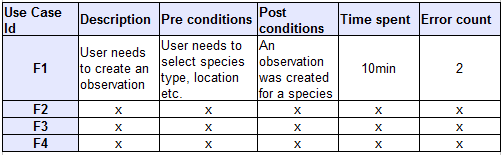
\includegraphics[scale=0.91]{reqspec/usabilitytable.png}
        \end{tabular}
        \label{tab:usecaseusability}
    \end{table}

Another method of measuring user attitude and perception towards a system is TAM.
TAM, technology acceptance model, is a tool with which users general perceived of use, perceived ease of use and intention to use is measured. While usability testing is more focused on  task based performance of users\cite{tam:doc4}, TAM is a general attitude test based on a twelve question model in which 3 things are measured

\begin{itemize}
\item PU - Perceived usefulness, how the user considers the system useful

\item PEU - Perceived ease of use, how the user considers the system easy to use
\item ITU - Intention to use, how likely is the user to want to use the system again
\end{itemize}

\begin{figure}[htb]
	\centering
	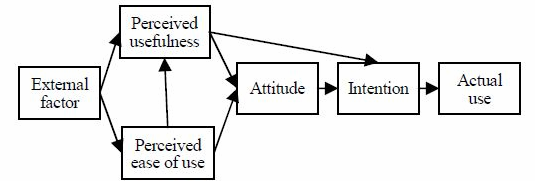
\includegraphics[width=0.7\textwidth]{reqspec/tam.png}
	\caption{Technology acceptance model framework\cite{tam:doc4}}
	\label{fig:tam}
\end{figure}

In this project, we will be using a revised version of the usability test we described above, especially focusing on effectiveness and efficiency. Artsdatabanken has an already web experienced user base and the number of novice users might probably not be significant to measure memorability and learnability of the system.
To measure performance and perception with regard to the system, the team will use a post questionnaire in the form of the three TAM categories. Learnability will also be explored using TAM.

%Perception test using a TAM Post questionnaire\cite{tam:doc4, tam:doc6}
\newpage
\paragraph{TAM}
Perception test using a TAM Post questionnaire\cite{tam:doc4, tam:doc6}, each designed to test the users attitude towards the new application.
    \begin{table}[!htb]
        \caption{TAM questionnaire items}
        \centering
        \begin{tabular}{cc}
        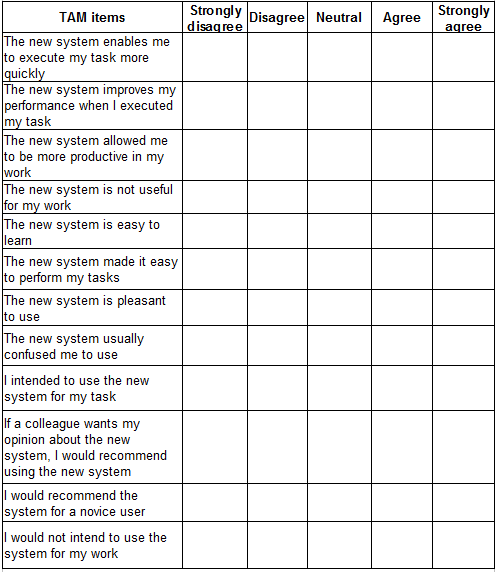
\includegraphics[scale=0.97]{reqspec/tamtable.png}
        \end{tabular}
        \label{tab:tam}
    \end{table}

The plan is to conduct a formal usability test using one of the fore mentioned methods  but the testing plan will be modified and restructured as our focus, goal and time resource changes. Usability testing can be extremely difficult to plan and to make sure the goals are met. Using a pilot test, organizing participants using standard methodology can be unrealistic for this  project. Because of this, we are going to make decisions that will suit the reality of this project and an actual documentation of the usability test result will be documented in section \ref{sec:testresult}.
\newpage

\subsubsection{Conclusions}

	QUnit provides a basic framework for synchronous and asynchronous testing in
	JavaScript, jquery-mockjax extends QUnit with the capability of mocking ajax
	requests and responsens. Selenium provides a comprehensive framework for
	automating tasks in the browser, as well as methods for inspecting the DOM.
	Using a combination of QUnit, jquery-mockjax, and Selenium we can
	efficiently use test-driven development in combination with PhoneGap.
